\documentclass{beamer}

\usepackage{color}			 % highlight
\usepackage{alltt}			 % highlight

\usepackage{tikz}
\usetikzlibrary{shapes,arrows,calc}
\tikzstyle{block} = [rectangle, draw, text width=5em, text centered]
\tikzstyle{arrow} = [draw, -latex']
\tikzstyle{line} = [draw]

\usepackage{pgfplots}
\pgfplotsset{compat=1.9}

\usepackage{hyperref}
\mode<presentation>

\title{Learn Haskell and R by doing Data Mining}
\author{Mihai Maruseac}

\setbeamertemplate{frametitle continuation}[from second]
%\setbeamertemplate{footline}[frame number]
\setbeamercolor{postit}{fg=black,bg=example text.fg!75!black!10!bg}

\renewcommand\quote[3]{
  \begin{beamercolorbox}[wd=\textwidth,rounded=true,shadow=true]{postit}
    #3
    \vskip5mm
    \hspace*\fill{\small{#1, \textit{#2}}}
  \end{beamercolorbox}
}

\pgfdeclareimage[height=3cm]{map}{img/filter-map}
\pgfdeclareimage[height=5cm]{folds}{img/folds}

\begin{document}

\maketitle

\begin{frame}{The Languages}
  \begin{description}
    \item[Haskell] functional programming, multipurpose
    \item[R] statistical computing and graphics
  \end{description}
\end{frame}

\begin{frame}{The Interpreter}
  \begin{description}
    \item[Haskell] \texttt{ghci}
      \begin{itemize}
        \item can compile with \texttt{ghc} (\texttt{-{}-make})
        \item can have build system: \texttt{cabal}
        \item \texttt{:l}, \texttt{:re}, \texttt{:t}, \texttt{:i}
      \end{itemize}
    \item[R] \texttt{R}
      \begin{itemize}
        \item compilable with special packages (\texttt{jit},
          \texttt{compiler})
        \item \texttt{source(file)}
      \end{itemize}
  \end{description}
\end{frame}

\begin{frame}{The Layout rules}
  \begin{description}
    \item[Haskell] indentation or curly braces and \texttt{;}
    \item[R] indentation or curly braces and \texttt{;}
  \end{description}
\end{frame}

\begin{frame}{The Types}
  \begin{description}
    \item[Haskell] static typing
      \begin{description}
        \item[Bool] \texttt{True} or \texttt{False}
        \item[Int] Integer (also \texttt{Integer}, \texttt{Float}, ..)
        \item[Char] Character
        \item[String] String (list of characters)
        \item[a] type variable
        \item[{[a]}] list of $a$s (types)
        \item[{(a, b)}] pair of an $a$ and a $b$ (type variables)
      \end{description}
    \item[R] dynamic typing
      \begin{itemize}
        \item \texttt{as.array}, \texttt{is.array}, \texttt{array}
      \end{itemize}
  \end{description}
\end{frame}

\begin{frame}{The Vectors (Lists, Arrays)}
  \begin{description}
    \item[Haskell] Lists only
      \begin{itemize}
        \item Vectors, etc. defined in packages
        \item Matrices: lists of lists (inefficient)
        \item constructors: \texttt{[]} and \texttt{:}
        \item \texttt{3 : [2, 4, 1]} is the same as \texttt{[3, 2, 4, 1]}
        \item \texttt{[1 .. 10]}, \texttt{[1, 3 .. 10]}, \texttt{[1..]}
        \item \texttt{head}, \texttt{tail}, \texttt{list !! index}
        \item \texttt{drop}, \texttt{take}
        \item \textbf{Lazy evaluation}
      \end{itemize}
    \item[R] construct everything from vectors (\texttt{array},
      \texttt{vector}, \texttt{list}, \texttt{dataframe}, \texttt{matrix})
      \begin{itemize}
        \item \texttt{c}, empty constructor, \texttt{1:10}
        \item only \texttt{1:10}
        \item \texttt{head}, \texttt{tail}, \texttt{vector[index]}
      \end{itemize}
  \end{description}
\end{frame}

\begin{frame}{Haskell :: More about Haskell Types}
  \begin{itemize}
    \item write your own type:
      \begin{itemize}
        \item type synonyms: \texttt{type String = [Char]}
        \item new data types: \texttt{data Type = Constructor ...}
        \item type variables in constructing types (think generics)\\
          \texttt{data Maybe a = Nothing | Just a}\\
          \texttt{data Either a b = Left a | Right b}
      \end{itemize}
    \item algebraic types:
      \begin{itemize}
        \item sum types: \texttt{data MyType = C1 Bool | C2 Char}
        \item product types: \texttt{(Bool, Char)} or \texttt{data MyType = C Bool Char}
        \item exponential types: functions
      \end{itemize}
  \end{itemize}
\end{frame}

\begin{frame}{The Functions}
  \begin{description}
    \item[Haskell]
      \begin{itemize}
        \item first class citizens (expressions)
        \item static typing: $a \rightarrow b$
        \item types as:
          \begin{itemize}
            \item documentation
            \item helpers
            \item proofs
          \end{itemize}
        \item \texttt{function arg1 arg2}
        \item \texttt{.} for function composition
        \item \texttt{f \$ x = f x}
        \item get rid of All parens!
      \end{itemize}
    \item[R]
      \begin{itemize}
        \item first class citizens too
        \item dynamic typing, use \texttt{is.*} and \texttt{as.*}
        \item \texttt{function(arg1, arg3=value)}
      \end{itemize}
  \end{description}
\end{frame}

\begin{frame}{Overloading}
  \begin{description}
    \item[Haskell] based on typeclasses (next slide)
    \item[R] redefine the function
  \end{description}
\end{frame}

\begin{frame}{Haskell :: Typeclasses}
  \begin{itemize}
    \item think Java interfaces
    \item methods available to all members of the class
  \end{itemize}
  \begin{beamercolorbox}[wd=\textwidth,rounded=true,shadow=true]{postit}
    \texttt{class Show a where\\
      \hspace{1em}show :: a -> String
    }
  \end{beamercolorbox}
  \pause
  \begin{beamercolorbox}[wd=\textwidth,rounded=true,shadow=true]{postit}
    \texttt{class Eq a where\\
      \hspace{1em}(==) :: a -> a -> Bool\\
      \hspace{1em}(/=) :: a -> a -> Bool\\
      \hspace{1em}x == y = not \$ x /= y\\
      \hspace{1em}x /= y = not \$ x == y
    }
  \end{beamercolorbox}
  \begin{itemize}
    \item but with default methods
  \end{itemize}
\end{frame}

\begin{frame}{Haskell :: Some Important Typeclasses}
  \begin{description}
    \item[{\texttt{Show}}] \texttt{show} (think \texttt{toString})
    \item[{\texttt{Read}}] \texttt{read}
    \item[{\texttt{Eq}}] \texttt{==} and \texttt{/=}
    \item[{\texttt{Ord}}] \texttt{compare}, \texttt{$<$}, $\ldots$
    \item[{\texttt{Enum}}]
    \item[{\texttt{Bounded}}]
    \item[{\texttt{Num}}]
    \item[{\texttt{Integral}}]
  \end{description}
\end{frame}

\begin{frame}{Haskell :: Registering Type to Typeclass}
  \begin{beamercolorbox}[wd=\textwidth,rounded=true,shadow=true]{postit}
    \texttt{
      data MyType = X .. | Y .. \color{red}{deriving (Eq, Show)}
    }
  \end{beamercolorbox}
  \pause
  \begin{beamercolorbox}[wd=\textwidth,rounded=true,shadow=true]{postit}
    \texttt{
      data MyType = X .. | Y .. \\
      \hspace{0.5em}\color{red}{instance Show MyType where}\\
      \hspace{1em}\hspace{1em}\color{blue}{show (X ..) = ..}\\
      \hspace{1em}\hspace{1em}\color{blue}{show (Y ..) = ..}
    }
  \end{beamercolorbox}
\end{frame}

\begin{frame}{The Ifs}
  \begin{description}
    \item[Haskell] \texttt{if e1 then e2 else e3}
      \begin{itemize}
        \item both branches needed
        \item \texttt{e1 :: Bool}
        \item \texttt{e2} and \texttt{e3} have same type
      \end{itemize}
    \item[R] same as in C, Java, etc.
  \end{description}
\end{frame}

\begin{frame}{The Loops}
  \begin{description}
    \item[Haskell] recursion or higher order functions
    \item[R] same as in C, Java, etc. or higher order functions (better
      avoided)
  \end{description}
\end{frame}

\begin{frame}{Haskell :: Higher Order Functions}
  \begin{center}
    \pgfuseimage{map}
  \end{center}
  \hspace{9em} \texttt{map} \hspace{5em} \texttt{filter}
\end{frame}

\begin{frame}{Haskell :: Higher Order Functions}
  \begin{center}
    \pgfuseimage{folds}
  \end{center}
  \hspace{9em} \texttt{foldr} \hspace{5em} \texttt{foldl}
\end{frame}

\begin{frame}{R :: Array ops}
  \begin{itemize}
    \item \texttt{names}, \texttt{colnames}, \texttt{rownames}
    \item ranges: \texttt{array[min:max]}
    \item range removals: \texttt{array[-min:-max]}
    \item item comparisons: \texttt{vector $\le$ bound}
    \item boolean selection: \texttt{vector[condition]}
  \end{itemize}
\end{frame}

\begin{frame}{Other interesting functions}
  \begin{description}
    \item[Haskell] \texttt{replicate}, \texttt{iterate}, \texttt{repeat},
      \texttt{dropWhile}, $\ldots$
    \item[R] \texttt{replicate}
  \end{description}
\end{frame}

\begin{frame}{Random number generation}
  \begin{description}
    \item[Haskell] \texttt{System.Random}
    \item[R] \texttt{sample}
  \end{description}
\end{frame}

\begin{frame}{Haskell :: Random}
  In \texttt{System.Random}
  \begin{itemize}
    \item \texttt{random :: (RandomGen g, Random a) => g -> (a, g)}
    \item \texttt{mkStdGen :: Int -> StdGen}
    \item \texttt{randomRs :: (RandomGen g, Random a) => (a, a) -> g -> [a]}
  \end{itemize}
\end{frame}

\begin{frame}[fragile]{Haskell :: random number generation}
\begin{verbatim}
import System.Random

data Bit = Zero | One deriving (Eq, Show, Enum, Bounded)

instance Random Bit where
  random g = (b, g') where
    (v, g') = randomR (0, 1) g
    b = if v == (0 :: Int) then Zero else One
  randomR (a, b) g = (x, g') where
    (y, g') = randomR (fromEnum a, fromEnum b) g
    x = toEnum y

getRandomBits :: StdGen -> Int -> [Bit]
getRandomBits g n = take n $ randomRs (minBound, maxBound) g
\end{verbatim}
\end{frame}

\begin{frame}{Distance metric}
  \begin{eqnarray*}
    d(x, y) & \ge & 0\\
    d(x, y) = 0 & \Leftrightarrow & x = y\\
    d(x, y) &=& d(y, x)\\
    d(x, y) & \le & d(x, z) + d(z, y)
  \end{eqnarray*}
\end{frame}

\begin{frame}{Distance ultrametric}
  \begin{eqnarray*}
    d(x, y) & \ge & 0\\
    d(x, y) = 0 & \Leftrightarrow & x = y\\
    d(x, y) &=& d(y, x)\\
    d(x, y) & \le & \max\{d(x, z),d(z, y)\}
  \end{eqnarray*}
\end{frame}

\begin{frame}{All triangles are issosceles}
  \begin{center}
    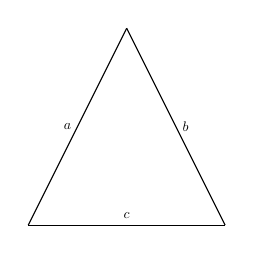
\begin{tikzpicture}[auto, scale=0.5, every node/.style={scale=0.5}]
      \draw [-] (0, 0) -- (2.5,5);
      \draw [-] (5, 0) -- (2.5,5);
      \draw [-] (5, 0) -- (0,0);
      \node at (1, 2.5) {$a$};
      \node at (4, 2.5) {$b$};
      \node at (2.5, .25) {$c$};
    \end{tikzpicture}
  \end{center}
  \pause
  \begin{eqnarray*}
    a & \ge & c\\
    b & \le & \max\{a, c\}\\
    b & \le & a\\
    a & \le & \max\{b, c\}
  \end{eqnarray*}
\end{frame}

\begin{frame}{Other relations}
  \begin{itemize}[<+->]
    \item all points in a sphere are centers of the sphere
    \item two spheres with a common point are the same sphere
  \end{itemize}
\end{frame}

\begin{frame}{Ultrametric clustering}
  \begin{enumerate}
    \item select a random item $x$ from the set of items
    \item for all other items $y$, compute $d(x, y)$
    \item all items $y$ closer to $x$ than a threshold $a$ form one cluster
    \item repeat all steps until there are no more items
  \end{enumerate}
\end{frame}

\begin{frame}{Tasks}
  \begin{enumerate}
    \item Write a function to generate an ADN sequence of $sz$ nucleotides
      ($A$, $C$, $G$, $T$)
    \item Write a function to generate $n$ sequences of size $sz$
    \item Write a function to compute the following distance between two
      sequences: if the nucleotide at position $i$ is different and all
      nucleotides before are equal then the distance is $2^{-i}$ (thus, a
      distance between 0 and 1)
    \item Do the clustering
  \end{enumerate}
\end{frame}

\end{document}
